\chapter{Experimental results}
These experimental results are shown the different performances when adapting mfcc feature in Audio-only ASR system and adapting video feature in Visual-only ASR system. As the tables below,it is clear to see, even both of the WERs are over 90\%, the audio-only system still has better performance than visual-only ASR system.
\begin{table}[ht]
\center
\begin{tabular}{c|c|c|c}

Model & Uni-gram & Bi-gram & Tri-gram\\ \hline
Mono &93.58\% &91.76\% & 92.68\%\\ 
Tri1 &92.94\% &91.77\% & 92.09\%\\ 
Tri2b &94.03\% &91.60\% & 93.02\% \\ 
Tri3b &92.39\% &90.22\% & 90.74\%\\ 
\end{tabular}
\caption{WER of Audio-only ASR system}
\label{tab:AWER}
\end{table}

\begin{table}[ht]
\center
\begin{tabular}{c|c|c|c}

Model & Uni-gram & Bi-gram & Tri-gram\\ \hline
Mono &98.49\% &98.82\% & 99.06\%\\ 
Tri1 &99.29\% &99.58\% & 99.67\%\\ 
Tri2b &99.58\% &99.48\% & 99.48\% \\ 
\end{tabular}
\caption{WER of Visual-only ASR system}
\label{tab:VWER}
\end{table}
Mono model is a model that using an mono-phone acoustic model to train features. While tri1 model use tri-phone acoustic model to train dynamic features with deltas + delta-delta, tri2b model use tri-phone acoustic model to train dimensional reduced features that handled by LDA and MLLT transformations. Tri3b is a Speaker Adapted Training, therefore, we don't train visual feature with this process.   
And to analyze these two tables respectively, we can see that the WERs are generally lower in Audio-only ASR system when they are adapted with bi-gram language model to decode. While in terms of Visual-only ASR system, we can not make any conclusion to connect the WER results with the n-gram language model. However, they are clear to show the effects of the acoustic models. No matter decode with any n-gram language model here, the WERs in the mono-phone acoustic model are usually lower than tri-phone model. 

Tri-phone models are context-dependent phone models, we adapt them because in different situations, even the same phoneme has different pronunciation.But among visual features, this problem does not exist and that make sense why visual-only system performs better when training with mono phone model.

\section{Analysis of Visual-only ASR system's result}
The experimental results are too bad with over 98\% WER, that is even worse than the audio-only ASR system. Audio features are not pure because it contains noise and instrument sound. In terms of visual-only ASR system, the bad result may arise from the quality of extracted features or the limited size of music corpus. To verify the assumptions, the following sections would analyze them.

\subsection{analysis of extracted visual pixel features}
As we know, the feature extraction is an vital step in ASR systems based on statistic models. The quality of the extracted features may have heavy impacts on the decoding result. In this section, we would plot the extracted visual pixel features to see whether they are in good quality.

From these continuous frames in utterance: F002\_002\_01\_0101.00.001, they are clear to show the lip\_region information.
\begin{center}
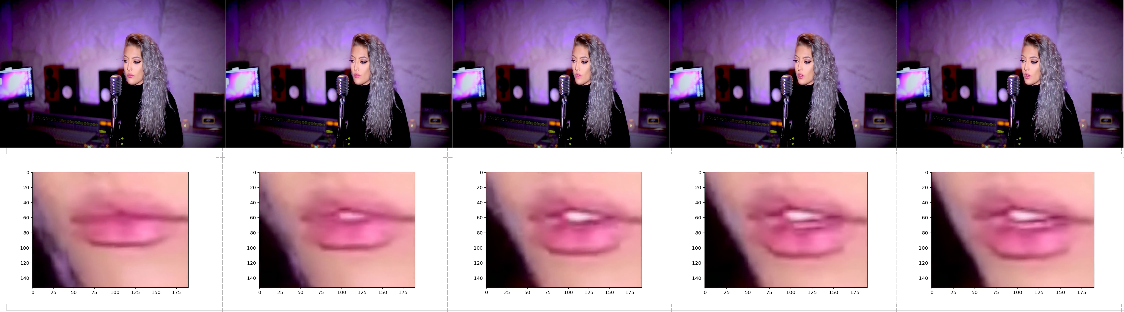
\includegraphics[width=0.8\linewidth]{images/F002.jpg}\\[1cm]
\label{img:F002}
\end{center}

However, the most extracted features\cite{2}} are not as good as the features above.
For example, in utterance : M020\_132\_01\_0101.00.027, the speaker moves his face quickly. As a result, the bounding box did not cover the ROI sometimes.
\begin{center}
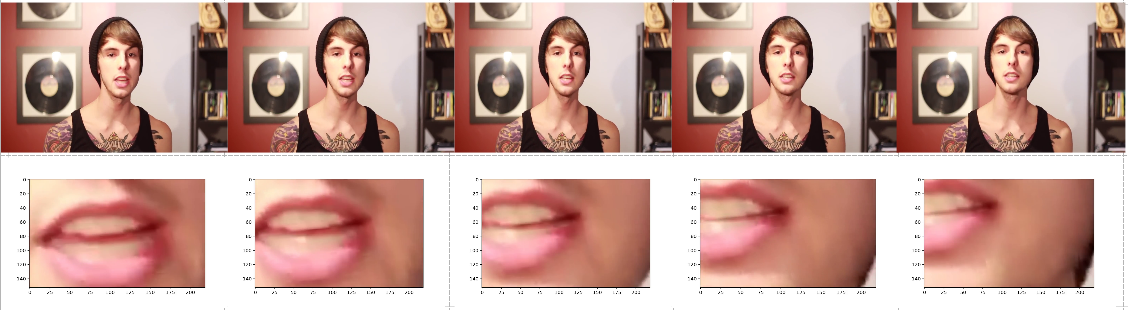
\includegraphics[width=0.8\linewidth]{images/M020.jpg}\\[1cm]
\label{img:M020}
\end{center}
In the following example, utterance-id : M001\_101\_01\_0101.00.022.
The extracted ROI features are bad because of the shelter of microphone.
\begin{center}
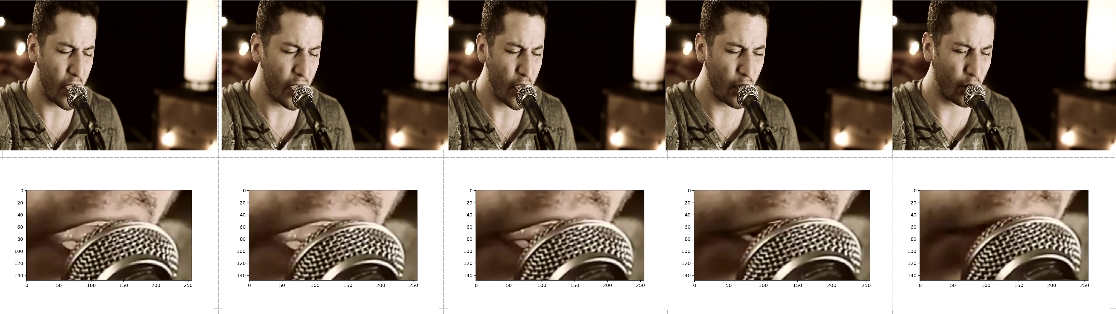
\includegraphics[width=0.8\linewidth]{images/M001.jpg}\\[1cm]
\label{img:M001}
\end{center}
While in this utterance M001\_001\_01\_0101.00.002 , the extracted features are more bad, since regardless of the shelter, the resolution of the video is low and may not able to show enough useful information.
\begin{center}
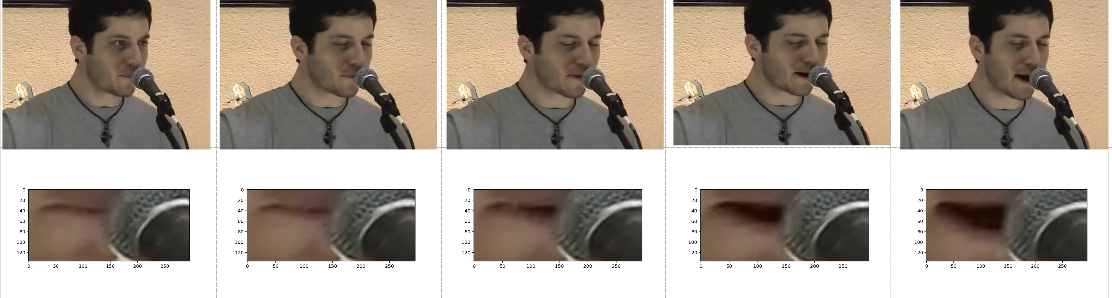
\includegraphics[width=0.8\linewidth]{images/M001_001.jpg}\\[1cm]
\label{img:M001_001}
\end{center}
Among these features, there is still another situation occurs in utterance M099\_044\_01\_0101.00.005. 
\begin{center}
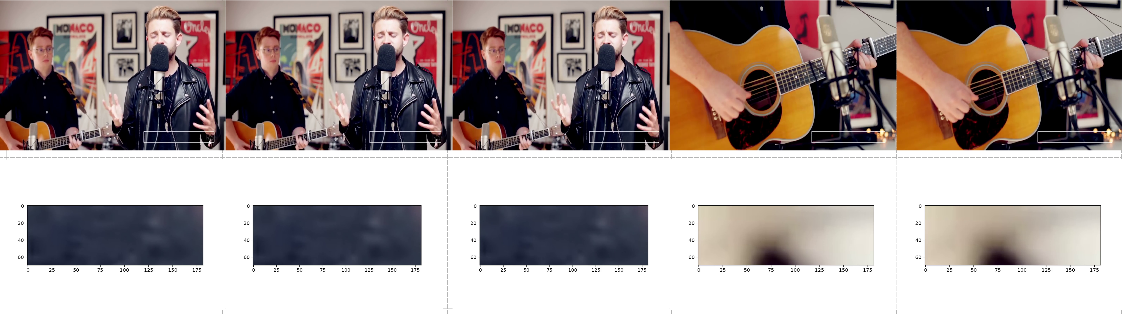
\includegraphics[width=0.8\linewidth]{images/M099.jpg}\\[1cm]
\label{img:M099}
\end{center}
The face detector in dlib toolkit mistaken the microphone as the detected face, and extract the part of it as lip region.
\begin{center}
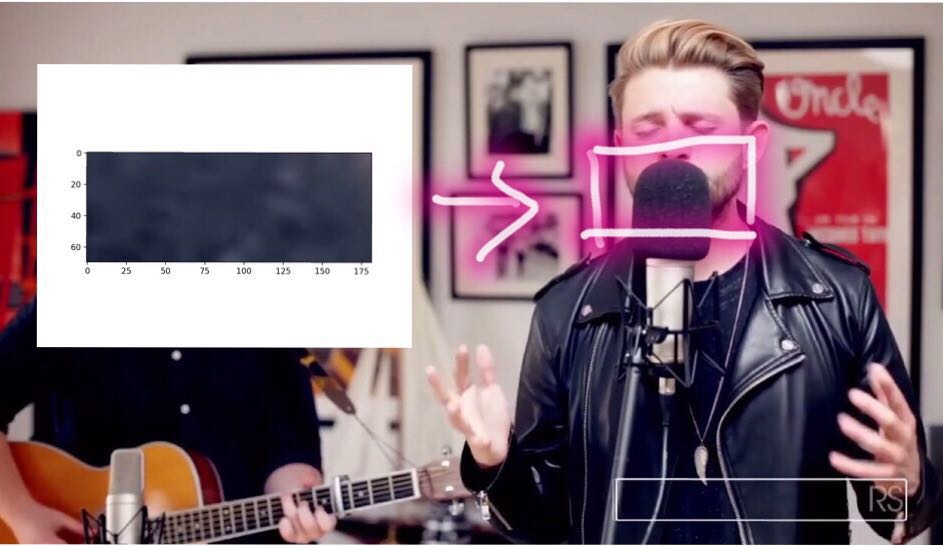
\includegraphics[width=0.6\linewidth]{images/bad1.jpg}\\[1cm]
\label{img:bad1}
\end{center}
\begin{center}
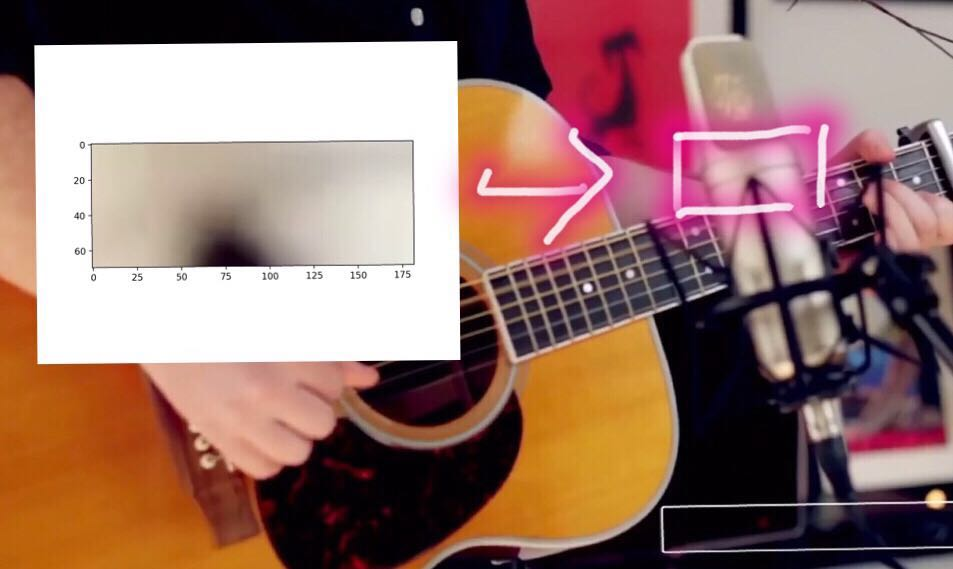
\includegraphics[width=0.6\linewidth]{images/bad2.jpg}\\[1cm]
\label{img:bad2}
\end{center}
The bad extracted features shown above may explain the reason why we got such bad WER results in visual-only ASR systems to some extent. To test whether the extracted features are still help in training the classifier. We
take the training set data also as the testing set and get the following results.
\begin{table}[ht]
\center
\begin{tabular}{c|c}

Model & WER\\ \hline
Mono &85.28\% \\ 
Tri1 &79.19\% \\ 
Tri2b &70.38\% \\ 

\end{tabular}
\caption{WER of Visual-only ASR system with training and testing on the same data set}
\label{tab:AWER}
\end{table}
This result is indeed a improvement and it reveals that the extracted visual features are still useful in training models.
\subsection{analysis of the size of music corpus}
As the table \ref{tab:utterance} shows, we just picked up 1013 utterances as a mini video corpus to build the visual-only ASR system. And among them only 615 utterances are for training , the left 398 utterances are taken as the testing set. Even though the WER results of Visual-only ASR system are more bad than Audio-only ASR system. We should notice that the audio-only ASR systems were trained and tested with 3428 utterances in total. Therefore, it is not reasonable to confirm which system performs better.


In the future, we should extend the useful video corpus in order to improve the Visual-only ASR system. Moreover, the algorithm of estimating lip region still can be improved, we should also focus on how to extract accurate visual features.

\section{Bad lip reading}

\textbf{Bad Lip Reading} is a YouTube channel,work to recompose films, TV shows, songs, sports, and political news stories by overdubbing humorous vocal that matches the lip movements of targets. It shows that, even audio-only front end system is weak in robust noise, visual-only front end system is also not reliable. Here are two videos, one is the original MV called \textbf{'you\'re beautiful'} from famous singer \textbf{James Blunt}, and the other is from this channel.
 
 These two videos\cite{3}} can be obtained on the website and the address would be appended in the following appendix. 




\section{Conclusion}
No matter ' lip reading for song transcription' or ' audio-only ASR in music', it is difficult to achieve results with low WER. For systems those already been built, it is hard to confirm whether the audio-only ASR system performs better or not, due to the different size of training data set.And in terms of visual-only ASR system, it could have a great improvement by extending the music corpus with good quality video files in extracting features. In the future, we can also focus on combing the audio front end with the visual front end to develop an AV-ASR system to see the performance.